\chapter{Patrones De Dise\~no}
	\section{Qu\'e Son Los Patrones De Dise\~no}
		Los patrones de dise\~no son la base para la b\'usqueda de soluciones a problemas comunes en el desarrollo de software y otros \'ambitos referentes al 
		dise\~no de interacci\'on o interfaces.
		Un patr\'on describe un problema que ocurre varias veces en un sistema, y la base de la soluci\'on a ese problema.
		Los patrones de dise\~no son el resultado del consenso de los profesionales en el \'area y brindan herramientas a los dise\~nadores de sistemas para no 
		escoger	malos caminos, vali\'endose de documentaci\'on disponible en lugar de simplemente la intuici\'on.
		
	\section{Patrones}
		Un patr\'on de dise\~no es una soluci\'on a un problema de dise\~no. Para que una soluci\'on sea considerada un patr\'on debe poseer ciertas 
		caracter\'isticas. Una de ellas es que se debe haber comprobado su efectividad resolviendo problemas similares en ocasiones anteriores. Otra es que debe 
		ser reusable, lo que significa que es aplicable a diferentes problemas de dise\~no en distintas circunstancias.
		Cada patr\'on de dise\~no se focaliza sobre un problema o issue particular de dise\~no (DOO).
		
		En general, un patr\'on tiene cuatro elementos esenciales:
		\begin{enumerate}
			\item \textbf{El nombre del patr\'on} es un manejador que se usa para describir un problema de dise\~no, su soluci\'on, y consecuencias.
			\item \textbf{El problema} describe cuando aplicar el patr\'on, explica el problema y su contexto. Tambi\'en describe problemas de dise\~no 
			espec\'ificos tales como \"Como representar un algoritmo como un objeto\". Adem\'as, describe la estructura de clases y objetos que son sintom\'aticas 
			de un dise\~no inflexible. A veces, el problema puede incluir una lista de condiciones que deben ser reunidas antes de que tenga sentido aplicar el 
			patr\'on.
			\item \textbf{La soluci\'on} describe los elementos que integran el dise\~no, sus relaciones, responsabilidades y colaboraci\'on. La soluci\'on no 
			describe un dise\~no particular concreto o implementaci\'on, porque un patr\'on puede ser aplicado en muchas situaciones diferentes. De hecho, el 
			patr\'on provee una descripci\'on abstracta de un problema de dise\~no y como una disposici\'on general de los elementos lo resuelve.  
			\item \textbf{Las consecuencias} son los resultados y compromisos de aplicar el patr\'on. Estas son fundamentales para evaluar alternativas de dise\~no 
			y para la comprensi\'on de los costos y beneficios de aplicar el patr\'on. Las consecuencias de un patr\'on incluye su impacto sobre la flexibilidad 
			del sistema, expansi\'on o portabilidad.
		\end{enumerate} 

	\section{Patrones Utilizados En \combeng}
		A lo largo del proceso de dise\~no se encontraron problemas que coincid\'ian con patrones. Estos patrones se explican brevemente a continuaci\'on: 
		
		\subsection{Observer}\label{patron_observer}
			Define una dependencia uno a muchos entre objetos, de forma que si un objeto cambia de estado, todos sus dependientes son notificados y 
			actualizados autom\'aticamente.
			En la Fig. \ref{pattern_observer} se ve el modelo est\'andar del patr\'on.
	 		\begin{figure}[ht]
				\centering
				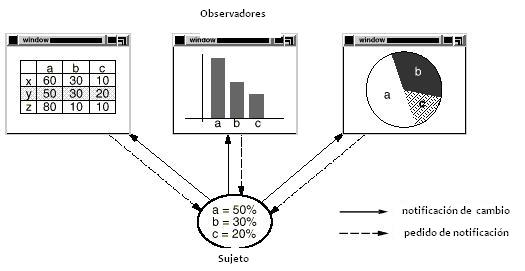
\includegraphics[scale=0.8]{images/pattern_observer.jpg}
				\caption{Patr\'on Observer.} \label{pattern_observer}
			\end{figure}

	    	\subsubsection{Aplicabilidad}
	    	Se usa el patr\'on $Observer$ cuando: 
		    \begin{itemize}
    			\item Una abstracci\'on tiene dos aspectos, uno dependiente del otro. Encapsular estos aspectos en objetos por separado le permite variarlo y 
    			reutilizarlos de manera independiente.
			    \item Un cambio de un objeto requiere cambiar a los dem\'as, y no se sabe cuantos objetos hay que cambiar.
				\item Un objeto debe ser capaz de notificar a otros objetos sin hacer suposiciones acerca de qu\'e son estos objetos. En otras palabras, no se 
				quiere que los objetos est\'en muy acoplados.
		    \end{itemize}
